%[Neste capítulo, cabe apresentar um resumo sobre o que já foi escrito sobre o tema para embasar teoricamente o presente projeto (já foram realizados trabalhos semelhantes? Qual o ponto de partida? Quais são os autores que serão consultados?).]

% There are good reasons to collect and track metrics. There are some really
% bad ones too. Anyone can use good metrics in terrible ways, such as using
% them as the basis for an individual team member’s performance evaluation.
% However, without metrics, how do you measure your progress?

% When metrics are used as guideposts—telling the team when it’s getting off
% track or providing feedback that it’s on the right track—they’re worth gath-
% ering. Is our number of unit tests going up every day? Why did the code cov-
% erage take a dive from 75\% to 65\%? It might have been a good reason —
% maybe we got rid of unused code that was covered by tests. Metrics can alert
% us to problems, but in isolation they don’t usually provide value.

[SEGUE UM EXEMPLO DE FUNDAMENTAÇÃO TEÓRICA USADO NO TRABALHO DE MEDIÇÃO E ANÁLISE]

Há alguns bons motivos para coletar e rastrear métricas, quando bem utilizadas. Métricas são interessantes para mensurar o progresso do código, porém podem ser vistas como anti-éticas para mensurar a performance de um membro em especial\cite{crispin2009agile}.

As métricas são importantes para rastrear motivos de, por exemplo, a cobertura caiu de 80\% pra 60\%, ou qual o motivo do \textit{velocity} do time decaiu em determinada semana.
Além de que, com as métricas é possível com o decorrer do tempo estimar e prever se a equipe terá chances de concluir determinado projeto em tempo, servindo assim como \textit{feedback} para a equipe e vindo a servir de motivação para a o desenvolvimento

\begin{quote}
	\textit{“There are three kinds of lies: lies, damned lies, and statistics.”}\\Benjamin Disraeli
\end{quote}

\begin{figure}[h]
	\centering
	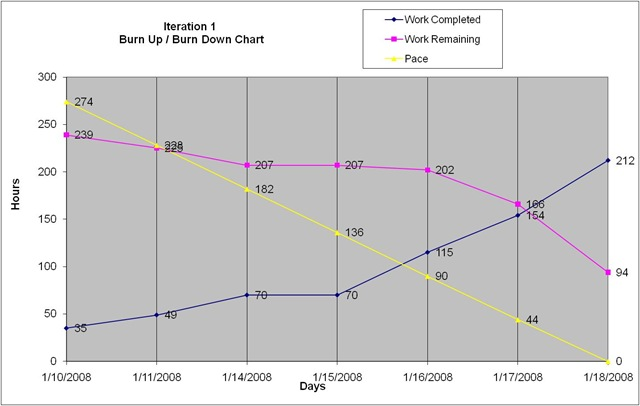
\includegraphics[width=0.6\textwidth]{conteudo/burnup}
	\caption{Exemplo de gráfico de \textit{Burn up \& Burn Down}\\ Fonte: One more Agile Blog\protect\footnotemark}
\end{figure}
\footnotetext{\label{imagem}Disponível em: <\url{http://www.onemoreagileblog.com/2009/07/common-agile-metrics.html}>. Acesso em 15 de outubro de 2014}

O uso das métricas  é valido quando há uma correta apresentação das mesmas, disponibilizando-as para a equipe e difundindo os pontos positivos da evolução da equipe. Logo, grandes gráficos expostos e de fácil compreensão são os melhores. Uma tabela extensa cheia de dados desordenados não é visivelmente atrativa e, mesmo que contenha uma densa quantidade de informações, pode se tornar menos informativa que um gráfico de linhas contendo os mesmos dados.

Segundo \cite{crispin2009agile}, pode vir a ser perigoso o uso de estatísticas na apresentação de métricas. Isso por que estatísticas são facilmente maleáveis, possibilitando que uma boa amostra seja apresentada como um ponto negativo ou pejorativo para algum membro da equipe. Uma possibilidade de uso de estatísticas é com visão do time todo por iterações ou \textit{releases}. Desta forma não há uma especificação do individuo, dificultando que possam ser apontados atores responsáveis por um possível baixo desempenho do time.


\begin{figure}[h]
	\centering
	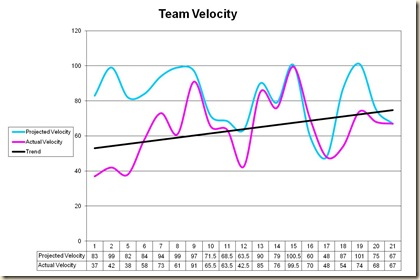
\includegraphics[width=0.5\textwidth]{conteudo/velocity}
	\caption{Exemplo de gráfico de \textit{Velocity}\\Fonte: One more Agile Blog\cref{imagem}}
\end{figure}

Em sistemas Linux, o uso de \textit{scripts} é recorrente e facilitam a automação de ações, deixando transparente para o usuário algumas interferências\cite{Advpdf}. Aproveitando o uso de ferramentas de integração continua, é possível gerar diversos relatórios que representam uma evolução detalhada do projeto. O uso combinado das ferramentas com \textit{scripts} de validação e retirada de métricas é bastante comum no desenvolvimento de aplicações nos dias atuais. Ferramentas como o Pylint podem ser utilizadas em curtos intervalos de desenvolvimento, providenciando métricas como cobertura e qualidade de código em números, o que possibilita a produção de gráficos informativos.
